\section{Second Stage}%
\label{s_second_stage}

Building on the baseline configuration of \cref{s_first_stage}, the
second stage of the process was executed and its output was recorded for
each of the four cases; the recorded response is shown in
\cref{fig:second_stage_response}. An example source is cited here only
to demonstrate that the bibliography compiles~\cite{example_source_2026};
delete this sentence and the corresponding \texttt{references.bib} entry
once a real report replaces this template.

\begin{figure}[!htb]
\centering
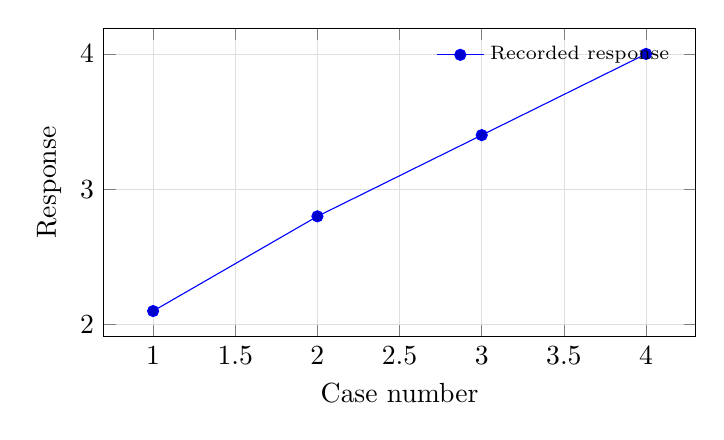
\begin{tikzpicture}
\begin{axis}[
  width=0.75\textwidth, height=5.5cm,
  xlabel={Case number}, ylabel={Response},
  grid=both, grid style={line width=0.2pt, draw=gray!25},
  legend style={font=\scriptsize, draw=none, fill=none},
]
\addplot+[mark=*] coordinates {(1,2.1) (2,2.8) (3,3.4) (4,4.0)};
\addlegendentry{Recorded response}
\end{axis}
\end{tikzpicture}
\caption{Recorded response of the second stage against case number, for
the baseline configuration of \cref{tab:baseline_config}. Values are
placeholders and should be replaced with the actual data supplied by the
caller.}
\label{fig:second_stage_response}
\end{figure}

\Cref{fig:second_stage_response} shows a monotonic increase in the
recorded response from case one through case four. This trend indicates
that the response scales with case number under the fixed baseline
configuration; whether the relationship is linear or the onset of a
higher-order effect should be stated explicitly once the real data
replaces this placeholder. The result motivates the discussion of case
sensitivity taken up in \cref{s_results}.
